\subsection{Overall accuracy of Simplified Ikeda method}
\label{se:overall_comparison}
An investigation of how well the implementation of the simplified Ikeda's method (see section \ref{se:semi-empirical methods}) agree with the corresponding results in the roll damping database has been carried out. 

Comparing roll damping is a bit difficult since the roll damping model consist of two coefficients, a linear term $B_1$ and a quadratic term $B_2$. These coefficients can be combined by calculating the equivalent linear damping coefficient for a certain roll angle $\phi_a$ \parencite{himeno_prediction_1981}:

\begin{equation}
B_{e} = B_{1} + \frac{8 B_{2} \omega_{0} \phi_{a}}{3 \pi}
\end{equation}

where $\phi_a$ was initially taken as the maximum roll angle from the roll decay tests. It was however found that a smaller value of 2 degrees gave better agreement and was instead used. For the roll damping database $B_1$ and $B_2$ can be inserted directly into the Eq. (\ref{eq:B_e_equation}) to get the equivalent roll damping $B_e$.

In order to obtain the same coefficients for the simplified Ikeda's method, roll damping was calculated for two or more roll amplitudes $\phi_a$ for the same motion frequency. $B_1$ and $B_2$ are obtained by fitting the Eq. (\ref{eq:B_e_equation}) to this data. The $B_e$ coefficient was made non-dimensional according to \parencite{himeno_prediction_1981} giving the non-dimensional equivalent linear damping coefficient $\hat{B_e}$, which was more convenient to use for this comparison as follows,
\begin{equation} \label{eq:be_eqvalent}
    \hat{B_e} = \frac{B_e}{\rho \bigtriangledown Beam^2} \sqrt{\frac{Beam}{2g}}
\end{equation}
where $\rho$, $\bigtriangledown$ and $Beam$ stand for fluid density, displacement volume and breadth of a ship, respectively.

It was found that almost all ships in the roll damping database were outside the limits that are suitable to be applied in Eq.(\ref{eq:SI_limits}). Two different ways to handle this limit exceedance was investigated: 1) the ``unlimited" approach where the input values are allowed to exceed the limits and 2) the ``limited" approach where the limit boundary values were used for exceeding values. Figure \ref{fig:ikeda_limited} show the comparison of roll damping predictions by the Simplified Ikeda's method using the ``unlimited" and ``limited" approach with the corresponding results from model tests. The ``limited" approach seems to be the best one to use according to this figure, where the ``unlimited" approach has values very far away from the model test results (as the red reference line).   
The large deviations with the ``unlimited" approach seem to originate from the wave damping coefficient $\hat{B_W}$ according to Fig. \ref{fig:ikeda_components}. Also the bilge keel damping coefficient $\hat{B_{BK}}$ seems to suffer from extrapolation when the ``unlimited" approach is used. 

\begin{figure}[H]
\vspace{-0.5cm}
\centering
  \centering
  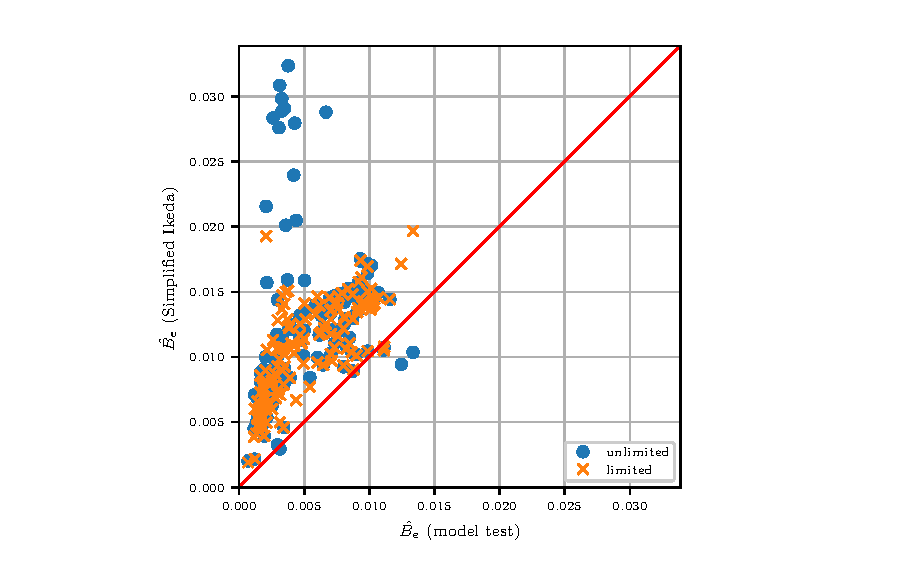
\includegraphics[height=5cm, width = 10cm]{figures/ikeda_limited.eps}
  \vspace{-0.5cm}
  \caption{$\hat{B_e}$ at all speeds estimated by the simplied Ikeda's method (Y-axis) in comparison with that from the roll decay test database (X-axis)}
  \label{fig:ikeda_limited}
\end{figure}


\begin{figure}[H]
\vspace{-0.5cm}
\centering
  \centering
  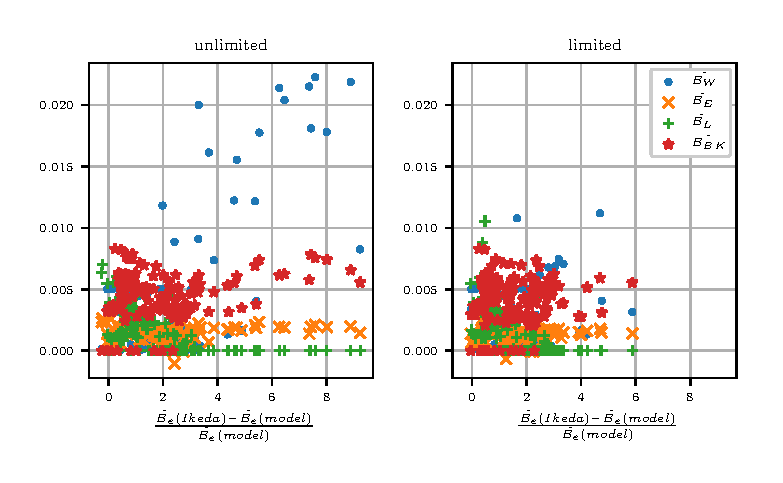
\includegraphics[height=6cm, width = 14cm]{figures/ikeda_components.eps}
  \vspace{-0.5cm}
  \caption{Investigation of how the roll damping components influence the error for the "unlimited" and "limited" approach to input extrapolation}
  \label{fig:ikeda_components}
\end{figure}



\textcolor{red}{\subsection{Improved S1 in literature?}}
\parencite[]{rudakovic_application_2017} has discovered that the eddy damping $ B_E $ becomes negative when $ C_b>0.84 $ (which is within the limits but close to the max limit 0.85). This has also been observed in the present comparison, which can be seen by some negative values in figure \ref{fig:ikeda_components}. These negative values are however small.

